\documentclass{beamer}
%
% Choose how your presentation looks.
%
% For more themes, color themes and font themes, see:
% http://deic.uab.es/~iblanes/beamer_gallery/index_by_theme.html
%
\mode<presentation>
{
  \usetheme{Boadilla}      % or try Darmstadt, Madrid, Warsaw, ...
  \usecolortheme{beaver} % or try albatross, beaver, crane, ...
  \usefonttheme{default}  % or try serif, structurebold, ...
  \useoutertheme{split}
  \setbeamertemplate{navigation symbols}{}
  \setbeamertemplate{caption}[numbered]
}

\usepackage[english]{babel}
\usepackage[utf8x]{inputenc}

\usepackage[font=tiny]{caption}

\title[Impl. and Visualization of the ChaCha Cipher Family in CT2]{Implementation and Didactical Visualization of the ChaCha Cipher Family in CrypTool 2}
\author{Ramdip Gill}
\institute{University of Heidelberg}
\date{January 28, 2021}

\setbeamertemplate{headline}{}
\setbeamertemplate{footline}
{
  \leavevmode%
  \hbox{%
  \begin{beamercolorbox}[wd=.2\paperwidth,ht=2.25ex,dp=1ex,center]{author in head/foot}%
    \usebeamerfont{author in head/foot}\insertauthor
  \end{beamercolorbox}%
  \begin{beamercolorbox}[wd=.6\paperwidth,ht=2.25ex,dp=1ex,center]{title in head/foot}%
    \usebeamerfont{title in head/foot}\insertshorttitle
  \end{beamercolorbox}%
  \begin{beamercolorbox}[wd=.2\paperwidth,ht=2.25ex,dp=1ex,right]{author in head/foot}%
    \usebeamerfont{date in head/foot} \insertframenumber{} / \inserttotalframenumber\hspace*{2ex}
  \end{beamercolorbox}
  }%
  \vskip0pt%
}

\urlstyle{same}

\begin{document}

\begin{frame}[plain]
  \titlepage
\end{frame}

% Uncomment these lines for an automatically generated outline.
\begin{frame}[plain]{Outline}
  \tableofcontents
\end{frame}

\section{Einleitung}

\subsection{CrypTool 2}
\begin{frame}{CrypTool 2}
\begin{figure}
\center
\begin{minipage}{.5\textwidth}
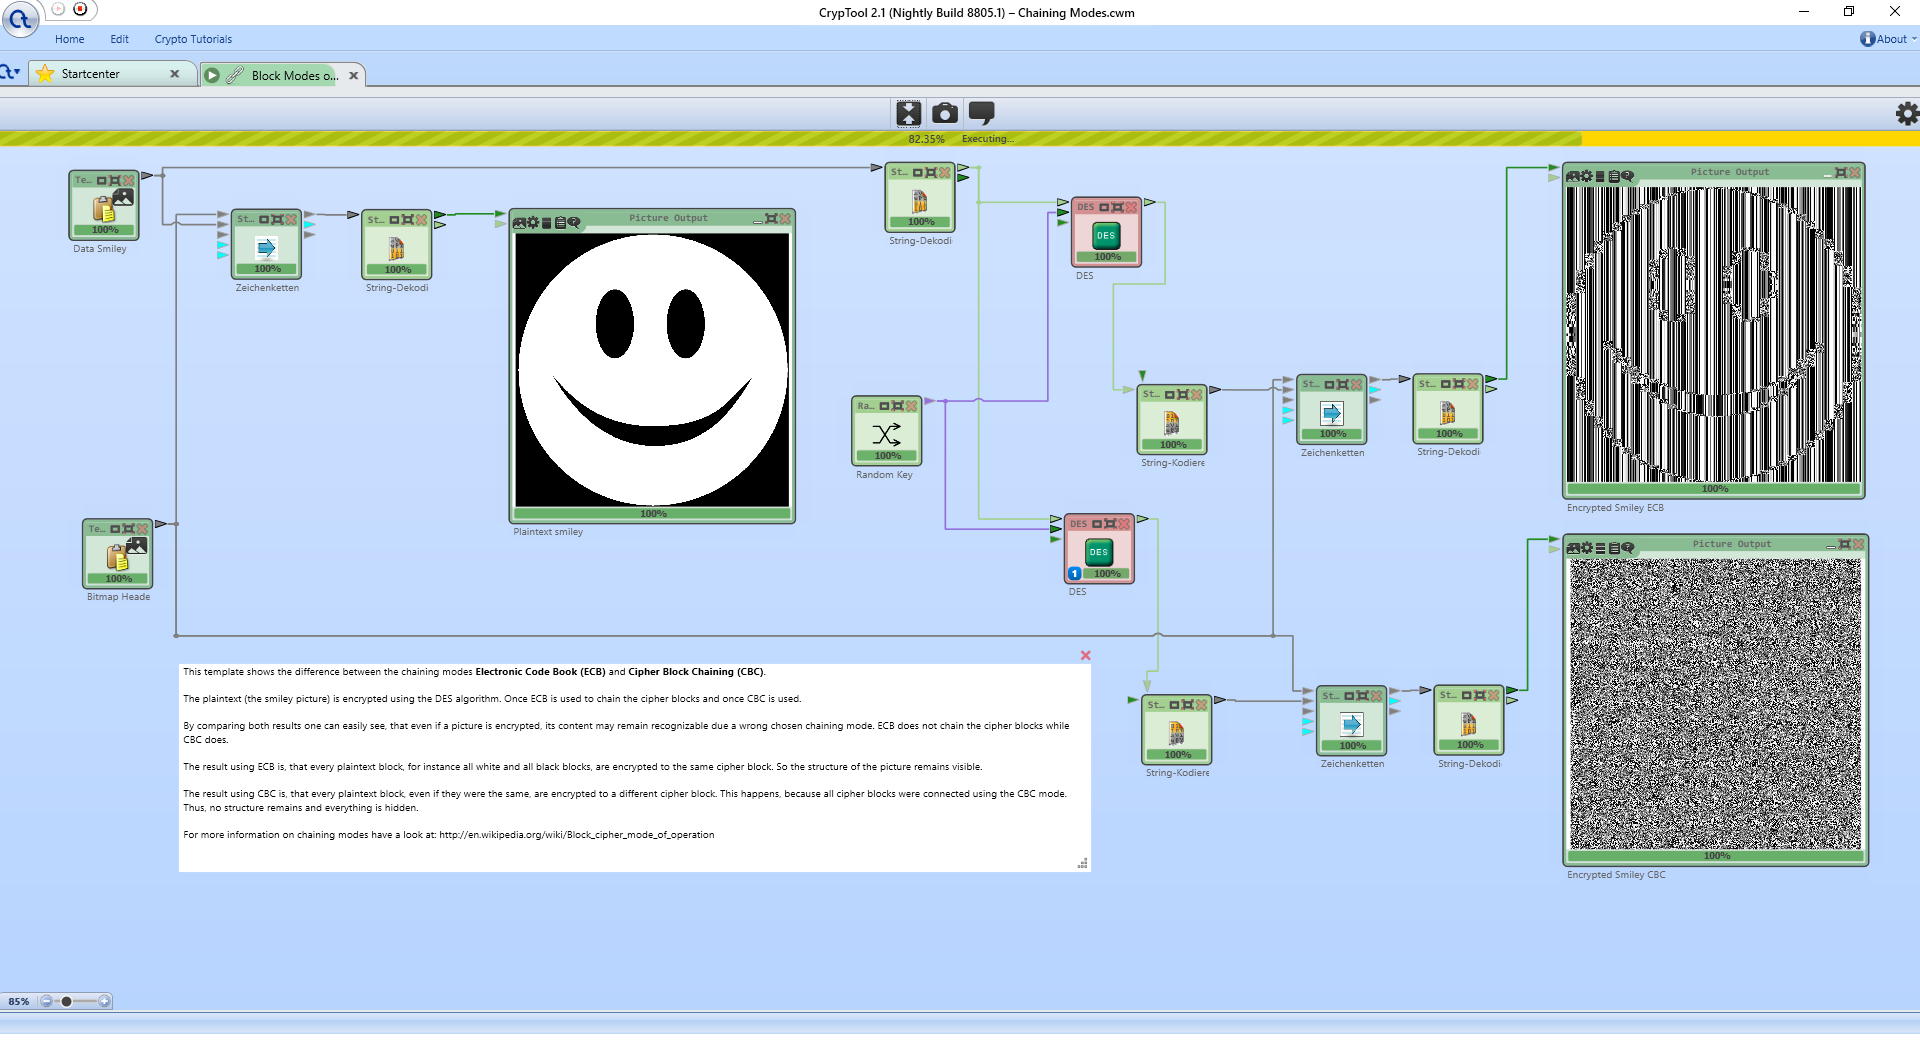
\includegraphics[width=\textwidth]{010_Block_Modes_Symmetric_Ciphers.png}
\caption{CrypTool 2: Demonstration Electronic Code Book (ECB) vs. Cipher Block Chaining (CBC) Modus}
\end{minipage}
\end{figure}
\begin{itemize}
\item kostenlose Open-Source E-Learning Platform \\für Kryptographie und Kryptoanalyse
\item benutzt Konzepte der visuellen Programmierung
\item beinhaltet unter anderem auch Visualisierungen \\von Chiffren wie AES, DES etc.
\item Kernteam von der Universität Siegen
\end{itemize}
\end{frame}

\subsection{ChaCha}
\begin{frame}{ChaCha}
\renewcommand*{\thefootnote}{\fnsymbol{footnote}}
\begin{itemize}
\item 256-bit Stromchiffre
\item veröffentlicht in 2008 von Daniel J. Bernstein
\item basiert auf Salsa20 des gleichen Authors
\item wird seit 2014 im Transport Layer Security Protokoll (TLS) \\eingesetzt aufgrund besserer Geschwindigkeit\footnotemark und Sicherheit gegenüber AES-GCM\\ $\Rightarrow$\ sehr relevant für moderne Kryptographie
\end{itemize}
\footnotetext[1]{in Software-Implementierungen}
\end{frame}

\section{Ziele des Plug-ins}
\begin{frame}{Ziele des Plug-ins}
\begin{itemize}
\item Unterstützung für 128-bit und 256-bit Schlüssel
\item Unterstützung für alle Chiffren der Familie (8, 12, 20 Runden)
\item Unterstützung für beide existierende Versionen: \\64-bit Zähler mit 64-bit Initialisierungsvektor (originale Version) und 32-bit Zähler mit 96-bit Initialisierungsvektor \\(Version der Internet Engineering Task Force)
\item Visualisierung des Ver-/Entschlüsselungsprozesses
\item Visualisierung der Diffusion
\item Fokus auf Didaktik
\end{itemize}
\end{frame}

\section{ChaCha Spezifikation}
\begin{frame}{ChaCha Spezifikation}

\begin{center}
\parbox{0.8\textwidth}{
\textbf{Abstract.} ChaCha8 is a 256-bit stream cipher based on the 8-round
cipher Salsa20/8. The changes from Salsa20/8 to ChaCha8 are designed
to improve diffusion per round, conjecturally increasing resistance to
cryptanalysis, while preserving—and often improving—time per round. [...]
\vspace{-0.75em}
\begin{flushright}
-- Daniel J. Bernstein
\end{flushright}
}
\end{center}
\begin{itemize}
\item Quelle: \url{https://cr.yp.to/chacha/chacha-20080120.pdf}
\item erläutert lediglich Unterschiede zu Salsa20
\item Unterschiede: Zustandsmatrix-Aufbau und Quarterround-Funktion
\end{itemize}
\end{frame}

\subsection{Aufbau der Zustandsmatrix}
\begin{frame}{Aufbau der Zustandsmatrix}
\end{frame}

\subsection{Quarterround-Funktion}
\begin{frame}{Quarterround-Funktion}
\end{frame}

\subsection{Hashfunktion}
\begin{frame}{Hashfunktion}
\end{frame}

\section{Live-Präsentation des Plug-ins}
\begin{frame}{Live-Präsentation des Plug-ins}
\end{frame}

\section{Architektur}
\begin{frame}{Architektur}
\end{frame}


\end{document}